% =====================================================================
%  BÁO CÁO ĐỒ ÁN CHUYÊN NGÀNH -- MẪU LaTeX (TIẾNG VIỆT)
%  Ho Chi Minh City University of Technology (HCMUT) - VNU-HCM
%  Biên dịch: pdflatex -> bibtex -> pdflatex -> pdflatex
%  (hoặc: latexmk -pdf main.tex; trên Overleaf chọn trình biên dịch pdfLaTeX)
% =====================================================================
\documentclass[vietnamese,final]{hcmut-thesis}

\usepackage{amsmath,amssymb}
\usepackage{booktabs}
\usepackage[nameinlink]{cleveref}   % dùng \Cref{} thay cho \ref{}

% ---------------------------------------------------------------------
%  Thông tin báo cáo -- CHỈNH SỬA Ở ĐÂY
% ---------------------------------------------------------------------
\reporttype{Đồ án chuyên ngành}
\title{Thời điểm truy hồi thích ứng: Học quyết định truy hồi mà không cần giám sát trực tiếp hay học tăng cường}
\stumajor{Khoa học Máy tính}
\supervisor{PGS.~TS.~Quản Thành Thơ}
\stuname{Nguyễn Phan Tuấn Duy -- 2310491}
\hypersetup{plainpages=false}
\setlength{\emergencystretch}{2em}

\begin{document}
\hypersetup{pageanchor=false}
\coverpage%
\hypersetup{pageanchor=true}

\frontmatter%
\begin{preface}{Lời cam đoan}
  Chúng tôi xin cam đoan đồ án chuyên ngành này là công trình do chúng tôi thực hiện dưới sự hướng dẫn của PGS. TS. Quản Thành Thơ tại Khoa Khoa học và Kỹ thuật Máy tính, Trường Đại học Bách khoa -- Đại học Quốc gia Thành phố Hồ Chí Minh.

  \noindent Mọi nguồn tài liệu và tham khảo bên ngoài được sử dụng trong đồ án đều đã được trích dẫn đầy đủ và rõ ràng.

  \noindent Nếu phát hiện có bất kỳ sự gian lận nào, chúng tôi xin hoàn toàn chịu trách nhiệm. Trường Đại học Bách khoa -- ĐHQG-HCM không liên quan đến những vi phạm tác quyền, bản quyền do chúng tôi gây ra (nếu có).

  \vspace{2cm}

  \begin{flushright}
    \begin{tabular}{c}
      \textit{\textbf{Nguyễn Phan Tuấn Duy}} \\
    \end{tabular}
  \end{flushright}
\end{preface}

\chapter*{Lời cảm ơn}
\addcontentsline{toc}{chapter}{Lời cảm ơn}
Em trân trọng cảm ơn PGS.\ TS.\ Quản Thành Thơ đã hướng dẫn thực hiện đề tài. Em xin cảm ơn quý thầy cô Khoa Khoa học và Kỹ thuật Máy tính, Trường Đại học Bách khoa, Đại học Quốc gia Thành phố Hồ Chí Minh, đã trang bị nền tảng chuyên môn cho quá trình học tập và thực hiện đồ án.

\chapter*{Tóm tắt}
\addcontentsline{toc}{chapter}{Tóm tắt}
Trong Multi-hop Question Answering (Multi-hop QA), bằng chứng cần thiết thường phụ thuộc vào kết quả của các bước suy luận trung gian. Retrieval-Augmented Generation (RAG) với lịch truy hồi cố định có thể bỏ sót bằng chứng hoặc thực hiện những lượt tìm kiếm không cần thiết. Đồ án khảo sát khả năng học thời điểm truy hồi thích ứng từ sự đánh đổi giữa Language Modeling Loss (LM Loss) và retrieval regularization, không cần nhãn trực tiếp cho từng quyết định truy hồi hay Reinforcement Learning.

Adaptive Retrieval Timing (ART) kết hợp Decision Head với Attention Mixing. Quy trình Collect--Replay cho phép truyền gradient từ hàm mục tiêu đến Decision Head trên quỹ đạo đã thu thập. Hai phép thăm dò H1 và H2 khảo sát cách supporting documents, distractor documents và mixing coefficient ảnh hưởng đến LM Loss và gradient, qua đó đánh giá các giả định nền tảng của phương pháp.

ART được đánh giá trên MuSiQue, HotpotQA và 2WikiMultiHopQA, mỗi benchmark gồm 500 câu hỏi. Tại retrieval threshold \(0.4297\), ART tăng F1 lần lượt \(20.92\), \(8.63\) và \(8.49\) điểm phần trăm so với Vanilla RAG. Threshold sweep cho thấy sự đánh đổi giữa chất lượng trả lời và số truy vấn. Kết quả này mô tả hiệu quả ở cấp hệ thống, bổ sung cho bằng chứng về tín hiệu học từ Attention Mixing.

\medskip\noindent\textbf{Từ khóa:} Adaptive Retrieval Timing, Multi-hop Question Answering, Retrieval-Augmented Generation, Attention Mixing, Collect--Replay.

\chapter*{Phân công công việc}
\addcontentsline{toc}{chapter}{Phân công công việc}
\begin{table}[htbp]
\centering
\begin{tabularx}{\linewidth}{@{}p{3.3cm}lX@{}}
\toprule
Sinh viên & MSSV & Phạm vi phần việc \\
\midrule
Nguyễn Phan Tuấn Duy & 2310491 & Nghiên cứu phương pháp, hiện thực cơ chế ART, kiểm chứng H1/H2, đánh giá đối chứng và tổng hợp kết quả giai đoạn DACN. \\
\bottomrule
\end{tabularx}
\end{table}


\tableofcontents
\clearpage
\listoffigures
\clearpage
\listoftables

\mainmatter%
\counterwithin{equation}{chapter}
\counterwithin{table}{chapter}
\counterwithin{figure}{chapter}

\chapter{Giới thiệu}
\label{chap:intro}
\section{Lý do chọn đề tài}
Trong hỏi đáp nhiều bước, mô hình có thể cần nhận diện một thực thể trung gian trước khi biết nên tìm bằng chứng nào tiếp theo. Một lượt truy hồi từ câu hỏi ban đầu có thể chỉ giải quyết mắt xích đầu tiên. Ngược lại, truy hồi quá thường xuyên đưa thêm distractor documents vào ngữ cảnh và làm tăng tải xử lý. Một pipeline RAG có thể phải thực hiện query rewriting, tạo embedding, vector search trên corpus lớn và reranking. Tùy thiết kế, các bước này có thể làm tăng tài nguyên sử dụng và latency. Đây là động lực nghiên cứu, còn tác động thực tế phụ thuộc vào hiện thực và cấu hình hệ thống.

\section{Phát biểu bài toán}
Cho câu hỏi \(q\), một kho đoạn văn và tiền tố sinh đến thời điểm \(t\), Decoder phải quyết định có cần truy hồi thêm trước khi tiếp tục sinh hay không. Thời điểm truy hồi là vị trí trong chuỗi sinh mà hệ thống đưa ra quyết định này. Ví dụ trong \cref{fig:baseline-case} cho thấy hai hệ thống xử lý cùng câu hỏi MuSiQue.

\begin{center}
\begin{minipage}{\linewidth}\centering
\setlength{\fboxsep}{6pt}\fbox{\begin{minipage}{.93\linewidth}
\textbf{Question}\par\nopagebreak[4]
{\small\ttfamily\raggedright
Who is the father of Nim\textquotesingle{}s actress in Return to Nim\textquotesingle{}s Island?\par
}
\textbf{Ground truth}\par\nopagebreak[4]
{\small\ttfamily\raggedright
Steve Irwin\par
}
\smallskip\hrule\smallskip
\textbf{No-RAG}\par\nopagebreak[4]
{\small\ttfamily\raggedright
François Civil\textless{}\textbar{}im\_end\textbar{}\textgreater{}\par
}
\textbf{Vanilla RAG}\par\nopagebreak[4]
{\small\ttfamily\raggedright
John Wayne\textless{}\textbar{}im\_end\textbar{}\textgreater{}\par
}
\smallskip\hrule\smallskip
\textbf{Vanilla RAG, passage 1}\par\nopagebreak[4]
{\small\ttfamily\raggedright
Title: Return to Nim\textquotesingle{}s Island\par
\textquotedbl{}Return to Nim\textquotesingle{}s Island\textquotedbl{}\par
Bindi Irwin as Nim Rusoe\par
}
\emph{[Lược phần còn lại; 4 đoạn khác không hiển thị.]}
\end{minipage}}
\captionof{figure}{Minh họa bài toán trên MuSiQue, ID 27. Câu hỏi, ground truth, raw outputs và đoạn trích lấy từ các bản ghi gốc.}
\label{fig:baseline-case}
\end{minipage}
\end{center}

No-RAG và Vanilla RAG đều không khớp đáp án chuẩn. Đoạn đứng đầu của Vanilla RAG nhận diện Bindi Irwin, một thực thể trung gian mà câu hỏi ban đầu chưa nêu tên. Bài toán đặt ra là học cách quyết định có nên truy hồi tiếp khi trạng thái sinh đã mang thêm thông tin.

\section{Mục tiêu}
Câu hỏi nghiên cứu là liệu mô hình có thể học thời điểm truy hồi từ sự đánh đổi giữa LM Loss và retrieval regularization, không cần nhãn trực tiếp hoặc Reinforcement Learning cho các quyết định truy hồi. Đồ án khảo sát tín hiệu nền tảng qua H1/H2, xây dựng phương pháp kết hợp Decision Head, Attention Mixing và Collect--Replay, rồi đánh giá hệ thống trên ba benchmark cùng threshold sweep.

\section{Phạm vi}
Đồ án chuyên ngành nghiên cứu thời điểm truy hồi cho Multi-hop QA, từ phép thăm dò đến đánh giá hệ thống. Lựa chọn công cụ và huấn luyện đồng thời retriever--generator thuộc phạm vi nghiên cứu tiếp theo của Đồ án tốt nghiệp.

\section{Đóng góp}
Đồ án chuyên ngành đóng góp một khảo sát thực nghiệm có kiểm soát về ảnh hưởng của bằng chứng và mixing coefficient lên LM Loss và gradient. Về phương pháp, đồ án kết nối điểm quyết định với Attention Mixing khả vi và xây dựng quy trình replay để học điểm này. Về hiện thực, hệ thống tích hợp truy hồi vào vòng sinh tự hồi quy và được so sánh với No-RAG và Vanilla RAG trên các mẫu ghép cặp. Đồ án dùng dữ liệu văn bản từ giáo viên để huấn luyện.

\section{Cấu trúc báo cáo}
\Cref{chap:background} trình bày nền tảng và công trình liên quan, \cref{chap:method,chap:implementation} mô tả phương pháp và hiện thực, \cref{chap:evaluation} phân tích thực nghiệm, và \cref{chap:conclusion} tổng kết.

\chapter{Cơ sở lý thuyết và các nghiên cứu liên quan}
\label{chap:background}
\section{Cơ sở lý thuyết}
Mô hình tự hồi quy phân rã xác suất văn bản thành tích các xác suất token có điều kiện trên tiền tố. Causal Attention giới hạn mỗi vị trí vào các key đã có. KV Cache lưu các phép chiếu key và value của tiền tố để tái sử dụng khi sinh token mới. Một quan sát chèn vào tiền tố có thể thay đổi phân bố của token kế tiếp.

Dense Retriever ánh xạ truy vấn và đoạn văn thành embedding. ART dùng E5 để tạo biểu diễn và FAISS để tìm các hàng lân cận trong chỉ mục\cite{e5,faiss}. Tìm kiếm trả về một danh sách hữu hạn các đoạn từ chỉ mục cố định. Vấn đề nghiên cứu ở đây là chọn thời điểm gọi bộ tìm kiếm trong vòng sinh.

\section{Các nghiên cứu liên quan}
RAG kết hợp mô hình sinh với kho tài liệu ngoài\cite{rag}. Vanilla RAG trong đồ án tìm một lần theo câu hỏi, trước khi sinh. IRCoT xen kẽ suy luận từng bước và tìm kiếm, dùng nội dung đã sinh để cải thiện truy vấn tiếp theo\cite{ircot}. Self-RAG học các reflection token để quyết định truy hồi và đánh giá bằng chứng hoặc câu trả lời\cite{selfrag}. R-Search dùng Reinforcement Learning với nhiều thành phần reward để tối ưu quỹ đạo xen kẽ suy luận và tìm kiếm\cite{rsearch}.

\begin{center}\begin{minipage}{\linewidth}\centering
\captionof{table}{Đối chiếu cơ chế chọn thời điểm truy hồi.}
\label{tab:signals}
\begin{tabularx}{\linewidth}{@{}p{2.5cm}XX@{}}
\toprule
Cách tiếp cận & Quyết định truy hồi & Tín hiệu cho cơ chế quyết định \\
\midrule
Vanilla RAG & Một lượt trước khi sinh & Quy tắc cố định \\
IRCoT & Xen kẽ theo bước suy luận & Bước suy luận đã sinh, theo quy trình xen kẽ \\
Self-RAG & Sinh reflection token & Giám sát các token phản tư \\
R-Search & Chính sách xen kẽ suy luận và tìm kiếm & Reward trong Reinforcement Learning \\
ART & Điểm từ trạng thái Decoder tại các biên ứng viên & LM Loss và retrieval regularization qua Collect--Replay \\
\bottomrule
\end{tabularx}
\end{minipage}\end{center}

\section{Tổng kết}
\Cref{tab:signals} phân biệt các cơ chế theo tín hiệu học và cách quyết định. ART tập trung vào câu hỏi phương pháp: liệu mục tiêu sinh có thể cung cấp tín hiệu gián tiếp cho retrieval timing thông qua Attention Mixing, kết hợp với một hình phạt đặt lên điểm quyết định. Hai phép thăm dò kiểm tra giả định cho đường học này; đánh giá benchmark đo kết quả ở cấp hệ thống.

\chapter{Phương pháp đề xuất}
\label{chap:method}
\section{Tổng quan hướng tiếp cận}
Với mỗi segment \(t\) gồm \(L\) token, Decoder Qwen2.5-3B-Instruct tạo các trạng thái ẩn và sử dụng trạng thái của token cuối cùng \(h_{t,L}\) làm đầu vào cho Decision Head. Thông qua phép chiếu tuyến tính và hàm sigmoid, Decision Head dự đoán điểm quyết định truy hồi:

\begin{equation}d_t = \sigma(w^\top h_{t,L} + b).\label{eq:gate}\end{equation}

Trong giai đoạn suy luận (inference), tại prefill và biên câu đủ điều kiện, hệ thống thực hiện truy hồi nếu truy vấn hợp lệ và \(d_t \geq \tau\). Khi truy hồi được thực hiện, điểm \(d_t\) được liên kết với quan sát mới và sử dụng làm hệ số Attention Mixing \(d\) trong các lần forward Decoder tiếp theo, cho đến khi quan sát đó được thay thế bởi kết quả truy hồi mới.

Đối với các thực nghiệm kiểm chứng giả thuyết H1/H2, hệ số \(d\) được thiết lập trực tiếp thay vì dự đoán thông qua Decision Head, nhằm khảo sát ảnh hưởng của Attention Mixing đến LM Loss và gradient.

\section{Dữ liệu}
\textbf{Dữ liệu kiểm chứng giả thuyết H1/H2.} Các thực nghiệm sử dụng mẫu Multi-hop QA từ MuSiQue với dữ liệu được tạo bởi teacher model, phân nhóm theo số bước suy luận và tỷ lệ tài liệu hỗ trợ so với tài liệu gây nhiễu. Trong mỗi điều kiện thực nghiệm, câu hỏi, tài liệu và đích dự đoán được giữ cố định, trong khi hệ số Attention Mixing được thay đổi có kiểm soát nhằm khảo sát sự biến thiên của LM Loss và gradient.

\textbf{Dữ liệu huấn luyện ART.} Dữ liệu huấn luyện được xây dựng từ tập huấn luyện MuSiQue. Teacher model Qwen3-8B tạo chuỗi đích ngoại tuyến với bốn ví dụ few-shot và hướng dẫn xử lý trường hợp bằng chứng chưa đầy đủ. Trong Collect–Replay, ART dùng chuỗi đích này để thu thập quỹ đạo truy hồi rồi tối ưu mô hình trên các tiền tố đã lưu.

\textbf{Dữ liệu đánh giá.} Hệ thống được đánh giá trên ba bộ dữ liệu Multi-hop QA gồm MuSiQue, HotpotQA và 2WikiMultiHopQA. Các mẫu đánh giá được tách khỏi dữ liệu huấn luyện và được sử dụng để so sánh ART với các baseline No-RAG và Vanilla RAG\cite{musique,hotpot,twowiki}.

\section{Phương pháp}
\subsection{Attention Mixing}
Từ cùng dòng trạng thái, hệ thống chiếu \(Q,K,V\), rồi tính hai biến thể RoPE cho truy vấn và khóa. Đặt \(C\) là mặt nạ nhân quả, \(D\) là mặt nạ khóa của đoạn quan sát mới nhất và \(m\) là chiều khóa. Hai phân bố là
\begin{align}
A_+ &= \operatorname{softmax}(Q_+K_+^\top/\sqrt{m}+C),\\
A_- &= \operatorname{softmax}(Q_-K_-^\top/\sqrt{m}+C+D),\\
O &= \operatorname{Dropout}\big(dA_++(1-d)A_-\big)V_+.
\label{eq:mix}
\end{align}
Nhánh trừ hiệu chỉnh vị trí sau đoạn che bằng độ dài đoạn. Hai nhánh dùng chung giá trị của dòng có tài liệu. Sau phép trộn là phép chiếu đầu ra. Nếu thiếu mặt nạ hoặc thiếu \(d\), dùng nhánh cộng. Với các phép chiếu cố định, phần khối lượng trực tiếp trên khóa bị che tỉ lệ với \(d\); sau nhiều lớp trạng thái trung gian cũng phụ thuộc \(d\). Nhánh trừ vẫn có thể chịu ảnh hưởng của quan sát cũ trong tiền tố.
\Cref{fig:attention} minh họa hai nhánh Attention Mixing dùng chung value. Cả hai nhận cùng trạng thái đầu vào.
\par\medskip\noindent
\begin{minipage}{\linewidth}
\captionsetup{hypcap=false}
\centering
\includegraphics[width=.72\linewidth]{graphics/attention-figure.pdf}
\captionof{figure}{Trộn hai phân bố chú ý từ cùng trạng thái. Nhánh trừ che quan sát mới nhất, trong khi hai nhánh dùng chung giá trị. Sơ đồ do đồ án dựng từ mã hiện thực.}
\label{fig:attention}
\end{minipage}\par\medskip
\subsection{Mục tiêu học và giả thuyết}
Mục tiêu của ART là học khi nào cần truy hồi từ sự đánh đổi giữa khả năng dự đoán chuỗi đích và một số hạng phạt trên điểm quyết định. Với các vị trí token đích hợp lệ \(\mathcal T\), hàm mục tiêu trong Replay có dạng
\begin{equation}
\mathcal{L}_{\mathrm{LM}}=-\frac{1}{|\mathcal{T}|}
\sum_{t\in\mathcal{T}}\log p_\theta(y_t\mid x_{<t}),\qquad
\mathcal{L}=\mathcal{L}_{\mathrm{LM}}+0.05\sum_{j\in J}d_j.
\label{eq:loss}
\end{equation}
Token câu hỏi và tài liệu truy hồi không thuộc \(\mathcal T\). LM Loss dùng chuỗi đích do teacher model sinh. \(J\) là đa tập các lượt cộng điểm trong Replay, kể cả khoản cộng ở nhánh kết thúc nếu được kích hoạt. Regularization phạt điểm cao; LM Loss tạo tín hiệu theo mức độ mà quan sát cải thiện dự đoán. Số hạng phạt không đếm số truy vấn.

Khi Replay, gradient từ dự đoán token đi qua Attention Mixing đến Decision Head; regularization cũng tác động trực tiếp lên các điểm được cộng. Optimizer cập nhật tham số mô hình. Các quyết định truy hồi rời rạc và tài liệu đã được xác định trong Collect. Cơ chế này cho phép khảo sát liệu hành vi truy hồi thích ứng có hình thành mà không cần nhãn thời điểm hay Reinforcement Learning.

H1 khảo sát LM Loss khi thay đổi hệ số trộn \(d\) dưới các tỷ lệ tài liệu hỗ trợ và gây nhiễu. H2 đo gradient theo hệ số được cung cấp trực tiếp để đánh giá hướng của tín hiệu học cục bộ. Hai phép thăm dò kiểm tra giả định nền tảng; đánh giá hệ thống hoàn chỉnh được trình bày riêng ở Chương~\ref{chap:evaluation}.

\chapter{Thiết kế và hiện thực hệ thống}
\label{chap:implementation}
\section{Yêu cầu hệ thống}
Hệ thống ART gồm Decoder tùy biến từ Qwen2, bộ truy hồi tài liệu, bộ phân đoạn câu trực tuyến và bộ điều phối huấn luyện. Bộ truy hồi sử dụng E5 để mã hóa truy vấn, kết hợp FAISS để tìm kiếm các đoạn văn liên quan. Quá trình mã hóa áp dụng tiền tố truy vấn E5, mean pooling theo attention mask và chuẩn hóa L2; các vector float32 được sử dụng để tìm kiếm trên CPU. Mỗi kết quả truy hồi được ánh xạ đến đoạn văn tương ứng trong corpus và cung cấp cho Decoder dưới dạng quan sát.

\section{Kiến trúc hệ thống}
\subsection{Chuẩn bị chuỗi và tập tham số}
Câu hỏi được định dạng theo mẫu hội thoại, trong khi chuỗi đích do teacher model sinh ra được nối với token EOS và mã hóa riêng với câu hỏi. Các token thuộc câu hỏi và nội dung tài liệu truy hồi được gán nhãn -100 để loại khỏi quá trình tính LM Loss. Bộ nạp dữ liệu kiểm tra kiểu chuỗi và loại bỏ các mẫu có chuỗi đích rỗng.

Checkpoint ART được sử dụng trong đánh giá được huấn luyện trong 0.75 epoch. Quá trình fine-tuning chỉ cập nhật 15 lớp Decoder cuối trong tổng số 36 lớp cùng với Decision Head; các lớp còn lại được đóng băng nhưng vẫn tham gia lan truyền thuận. Kích thước micro-batch là 1, với gradient accumulation qua 32 bước.

\section{Quy trình Collect--Replay và suy luận}
\Cref{fig:workflow-overview} trình bày tổng quan ba giai đoạn hoạt động của ART.

\par\medskip\noindent
\begin{minipage}{\linewidth}
\centering
\captionsetup{hypcap=false}
\includegraphics[width=0.75\textwidth,keepaspectratio]{graphics/art-retrieval-workflow-approved.png}
\captionof{figure}{Sơ đồ tổng quan quy trình hoạt động của ART.}
\label{fig:workflow-overview}
\end{minipage}\par

\subsection{Collect--Replay khi training}
Collect–Replay tách bước chọn quỹ đạo truy hồi rời rạc khỏi bước tối ưu có gradient.

\textbf{Collect.} ART nạp câu hỏi, rồi xử lý chuỗi đích theo segment. Tại các điểm ứng viên, mô hình so sánh điểm mới \(d_t\) với ngưỡng. Ở các biên câu đủ điều kiện, exploration cũng có thể kích hoạt truy hồi. Collect chạy trong \texttt{no\_grad}, lưu tiền tố, attention masks, điểm và ngữ cảnh theo quỹ đạo. Nội dung quan sát lấy từ bộ truy hồi được chèn vào tiền tố, căn chỉnh với nhãn bỏ qua.

\textbf{Replay.} Mô hình chạy lại các tiền tố đã lưu mà không dùng KV Cache, tính lại điểm quyết định trong đồ thị gradient và ghép các phần logits mới theo thứ tự chuỗi. Quá trình này giữ nguyên tài liệu đã thu thập, tính \cref{eq:loss} và backpropagate. Quỹ đạo có thể kết thúc bằng một bản ghi chỉ chứa quyết định; nhánh này có thể cộng điểm cuối lần nữa và không đồng nghĩa truy hồi.

\subsection{Inference tự hồi quy}
Ở prefill, ART khởi tạo ngữ cảnh và KV Cache. Trong các bước sinh sau, mô hình kiểm tra biên câu và chỉ tính điểm ứng viên tại các vị trí đủ điều kiện. Khi \(d_t\geq\tau\), hệ thống lấy câu hoàn chỉnh gần nhất hoặc câu hỏi gốc làm truy vấn và kiểm tra dấu hiệu bị chặn. Nếu chấp nhận, ART truy hồi, chèn quan sát, cập nhật document mask và đồng bộ cache nhánh thứ hai từ nhánh có quan sát. Điểm vừa chấp nhận trở thành hệ số trộn cho quan sát mới. Nếu không truy hồi, hệ thống giữ ngữ cảnh đang hoạt động và tiếp tục sinh. Inference không dùng exploration.

\Cref{fig:workflow} đối chiếu các nhánh quyết định ở Collect và inference, cùng đường truyền gradient trong Replay.
\par\medskip\noindent
\begin{minipage}{\linewidth}
\centering
\captionsetup{hypcap=false}
\includegraphics[width=\linewidth]{graphics/workflow-figure.pdf}
\captionof{figure}{Sơ đồ kỹ thuật quy trình Collect--Replay và suy luận của ART.}
\label{fig:workflow}
\end{minipage}\par

\chapter{Thực nghiệm và đánh giá}
\label{chap:evaluation}
\section{Thiết lập thực nghiệm}
\subsection{Hai phép thăm dò cơ chế}
Để kiểm chứng hai giả thuyết H1 và H2, chúng tôi sử dụng Attention Mixing Probe, một phiên bản Decoder Qwen2.5 cho phép cung cấp trực tiếp tài liệu và hệ số trộn chú ý \(d\). Việc sử dụng tài liệu có sẵn giúp khảo sát riêng tác động của Attention Mixing, không phụ thuộc vào Decision Head hoặc quá trình truy hồi tự hồi quy.

Dữ liệu thí nghiệm được xây dựng từ các tập xác thực MuSiQue với câu hỏi yêu cầu 2, 3 và 4 bước suy luận. Dựa trên nhãn đoạn hỗ trợ của bộ dữ liệu, mỗi mẫu được cung cấp ba đoạn văn theo bốn cấu hình: 0:3, 1:2, 2:1 và 3:0, tương ứng với số đoạn hỗ trợ và đoạn gây nhiễu. Các đoạn được lấy mẫu một lần cho mỗi câu hỏi với seed 42 và được giữ cố định khi thay đổi hệ số trộn. Cả hai phép thăm dò đều khảo sát 33 giá trị \(d=i/32\), với \(i=0,\ldots,32\).

Đối với H1, mô hình được chạy ở chế độ suy luận để đo LM Loss trên các token đích tại từng giá trị \(d\). Đối với H2, các tham số mô hình được đóng băng và gradient của LM Loss theo hệ số \(d\) được ghi nhận thông qua hook, không thực hiện cập nhật tham số (learning rate bằng 0). Kết quả được tổng hợp trên 1.024 mẫu đối với các cấu hình 0:3, 1:2 và 2:1; riêng cấu hình 3:0 có 494 mẫu do điều kiện 2 bước không đủ ba đoạn hỗ trợ. Vì vậy, khi so sánh kết quả giữa các cấu hình, cần lưu ý sự khác biệt về thành phần mẫu và lượng thông tin hỗ trợ được cung cấp.

\subsection{Đối chứng hệ thống}
Để đánh giá hiệu quả của hệ thống ART, chúng tôi tiến hành thực nghiệm trên ba bộ dữ liệu MuSiQue, HotpotQA và 2WikiMultiHopQA, mỗi bộ gồm 500 mẫu. Ba phương pháp được đánh giá trên cùng tập câu hỏi và đáp án tham chiếu nhằm bảo đảm tính nhất quán trong quá trình so sánh.

Các phương pháp đối chứng bao gồm:

\begin{itemize}
\item \textbf{No-RAG:} Mô hình sinh câu trả lời trực tiếp từ câu hỏi mà không sử dụng tài liệu truy hồi.
\item \textbf{Vanilla RAG:} Mô hình truy hồi một lần dựa trên câu hỏi ban đầu, sử dụng 5 đoạn văn liên quan để hỗ trợ sinh câu trả lời.
\item \textbf{ART:} Hệ thống quyết định thời điểm truy hồi trong quá trình sinh, với 5 đoạn văn được lấy ở mỗi lượt truy hồi.
\end{itemize}
Cả ba phương pháp đều sử dụng kiến trúc nền Qwen2.5-3B-Instruct. Tuy nhiên, No-RAG và Vanilla RAG sử dụng checkpoint gốc, trong khi ART sử dụng checkpoint đã fine-tune. Vì vậy, kết quả so sánh phản ánh hiệu quả tổng thể của hệ thống ART, bao gồm cả quá trình fine-tuning và cơ chế truy hồi thích nghi, thay vì chỉ đo lường riêng tác động của việc lựa chọn thời điểm truy hồi.

Hiệu quả trả lời câu hỏi được đánh giá thông qua ba chỉ số Accuracy (Acc), Exact Match (EM) và token-level F1, sử dụng quy tắc chuẩn hóa và so khớp đáp án theo bộ đánh giá R-Search. Kết quả được tính trung bình trên toàn bộ mẫu và biểu diễn dưới dạng phần trăm.

Trong evaluator, Acc đo tỷ lệ dự đoán chứa ít nhất một đáp án tham chiếu dưới dạng chuỗi con, không phân biệt hoa thường. EM và F1 so khớp sau chuẩn hóa. Các quy tắc này khớp với mã đánh giá R-Search\cite{rsearch}.

\section{Kết quả}
\subsection{Kiểm chứng H1 và H2}
\textbf{H1.} \Cref{fig:h1} cho thấy LM Loss thay đổi theo hệ số trộn \(d\) và tỷ lệ tài liệu hỗ trợ so với tài liệu gây nhiễu. Khi cả ba tài liệu đều gây nhiễu (0:3), tăng \(d\) ban đầu chỉ làm LM Loss giảm nhẹ từ 1.3160 tại \(d=0\) xuống 1.2753 tại \(d=0.25\). Sau đó, LM Loss tăng lên 1.3943 tại \(d=1\). Khi có tài liệu hỗ trợ, LM Loss giảm rõ hơn. Các giá trị thấp nhất quan sát được với tỷ lệ 1:2, 2:1 và 3:0 lần lượt là 1.1295, 0.9495 và 0.8830, tại \(d\) xấp xỉ 0.656, 0.719 và 0.750.

Hiệu quả của Attention Mixing phụ thuộc vào thành phần bằng chứng. Tài liệu hỗ trợ có thể giúp giảm LM Loss, trong khi tài liệu gây nhiễu hạn chế lợi ích đó. Cả bốn đường đều tăng trở lại khi \(d\) tiến đến 1, cho thấy sử dụng tối đa thông tin truy hồi không nhất thiết có lợi nhất trong thí nghiệm. LM Loss được đo dưới teacher forcing nên chưa trực tiếp cho biết chất lượng câu trả lời khi mô hình sinh tự do. Ngoài ra, điều kiện 3:0 thiếu dữ liệu hai bước, nên cần thận trọng khi so sánh với các nhóm còn lại.
\begin{figure}[htbp]\centering
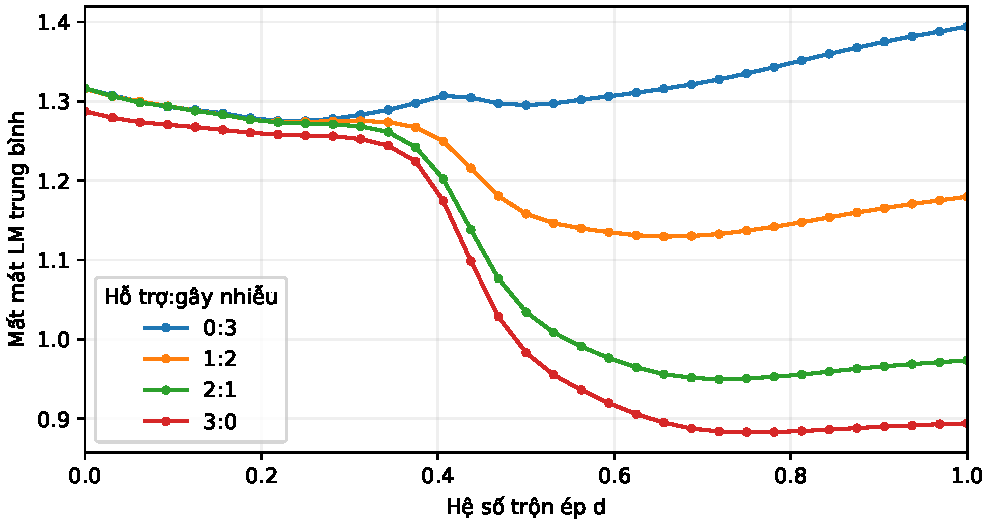
\includegraphics[width=.86\linewidth]{graphics/h1.pdf}
\caption{H1: mất mát trung bình trên đích theo hệ số trộn ép và tỷ lệ hỗ trợ:gây nhiễu. Nguồn: tổng hợp H1 của đề tài.}
\label{fig:h1}
\end{figure}

\pagebreak[4]
\textbf{H2.} \Cref{fig:h2,fig:h2cost} khảo sát gradient của LM Loss theo hệ số trộn \(d\). Gradient âm cho biết tăng nhẹ \(d\) có xu hướng làm giảm LM Loss tại điểm đang xét. Gradient dương cho biết tăng nhẹ \(d\) có xu hướng làm tăng LM Loss. Như vậy, độ dốc cung cấp tín hiệu cục bộ để mô hình học cách điều chỉnh mức sử dụng thông tin truy hồi.

Điều kiện chỉ chứa tài liệu gây nhiễu (0:3) có gradient dương lớn nhất tại \(d=0.375\), còn ba điều kiện có tài liệu hỗ trợ đạt gradient âm nhỏ nhất tại \(d=0.4375\). Sự khác biệt này gợi ý khảo sát vùng \(d\) khoảng 0.40--0.44, nơi tín hiệu gradient có thể phản ánh sự khác nhau giữa bằng chứng hỗ trợ và bằng chứng gây nhiễu. Gradient thay đổi theo \(d\), và tại \(d=1\) cả bốn điều kiện đều có gradient dương. Do đó, kết quả chưa cho thấy một giá trị \(d\) cố định phù hợp với mọi trường hợp.

Để khảo sát ảnh hưởng của chi phí truy hồi, \cref{fig:h2cost} minh họa điều kiện \(g(d)+\lambda=0\) qua các đường tham chiếu \(-\lambda\), với \(\lambda\) lần lượt bằng \(0\), \(0.05\) và \(0.1\). Các giao điểm cho biết những vị trí mà độ dốc của hàm mục tiêu có thể đổi dấu trong miền khảo sát. Chúng không xác định trực tiếp ngưỡng truy hồi tối ưu.

Trong thí nghiệm H1--H2, \(d\) là hệ số trộn được đặt trước. Khi mô hình sinh tự do, \(d_t\) là đầu ra của Decision Head. ART dùng ngưỡng vận hành \(\tau=0.4297\) theo kinh nghiệm để so sánh với \(d_t\). Các đồ thị H1--H2 không chứng minh đây là ngưỡng tối ưu.
\begin{figure}[htbp]\centering
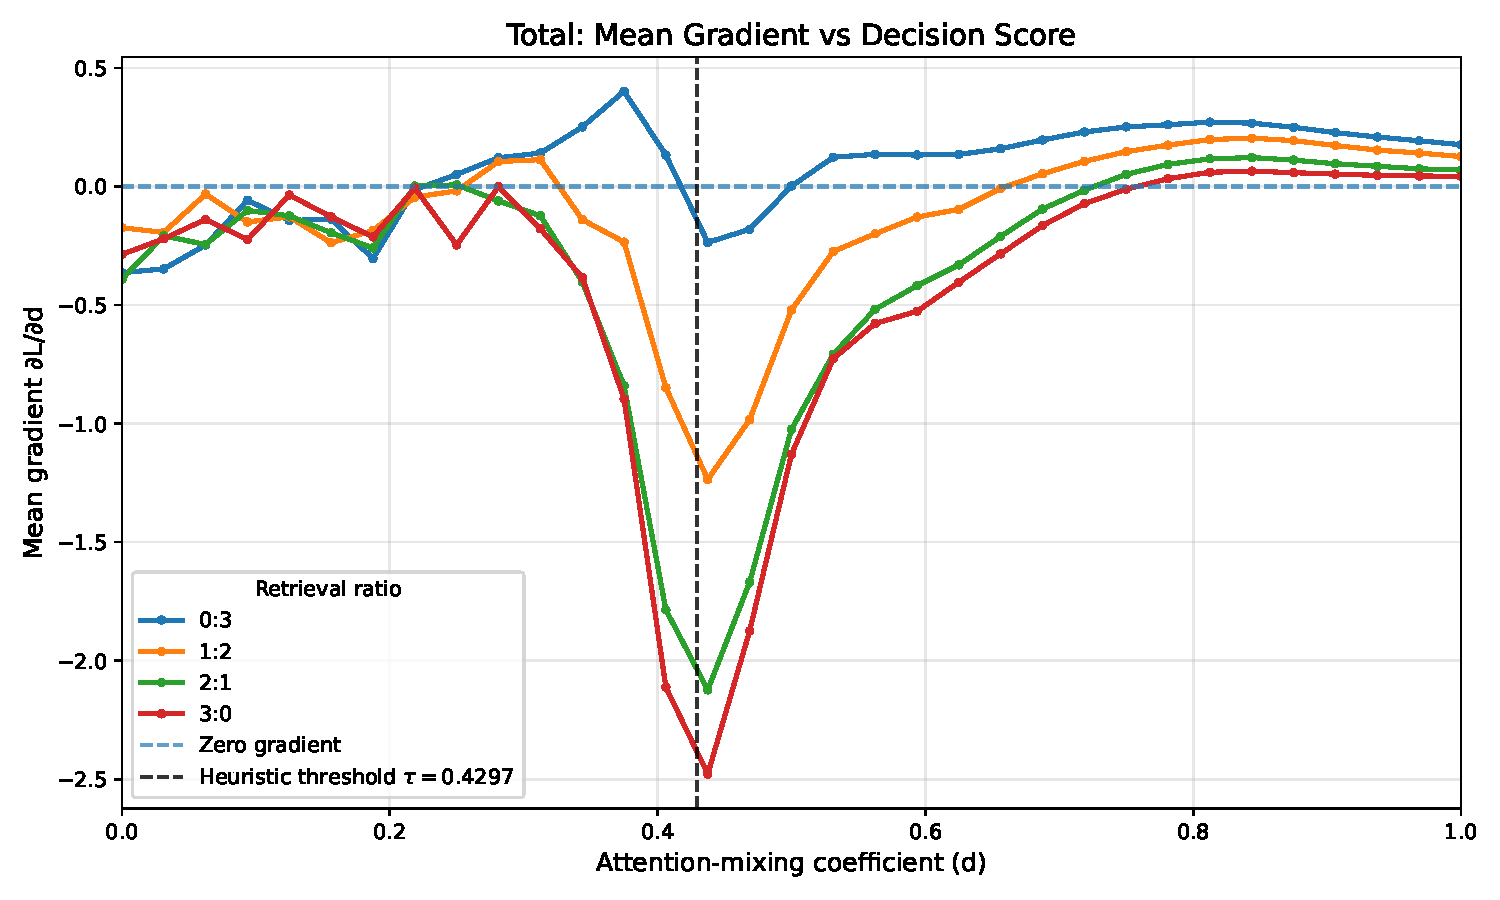
\includegraphics[width=.86\linewidth]{graphics/h2-gradient.pdf}
\caption{H2: gradient mất mát trung bình theo \(d\). Vạch đứng chỉ ngưỡng vận hành \(\tau\) để tham chiếu. Nguồn: notebook H2, ô vẽ đường gradient.}
\label{fig:h2}
\end{figure}
\begin{figure}[htbp]\centering
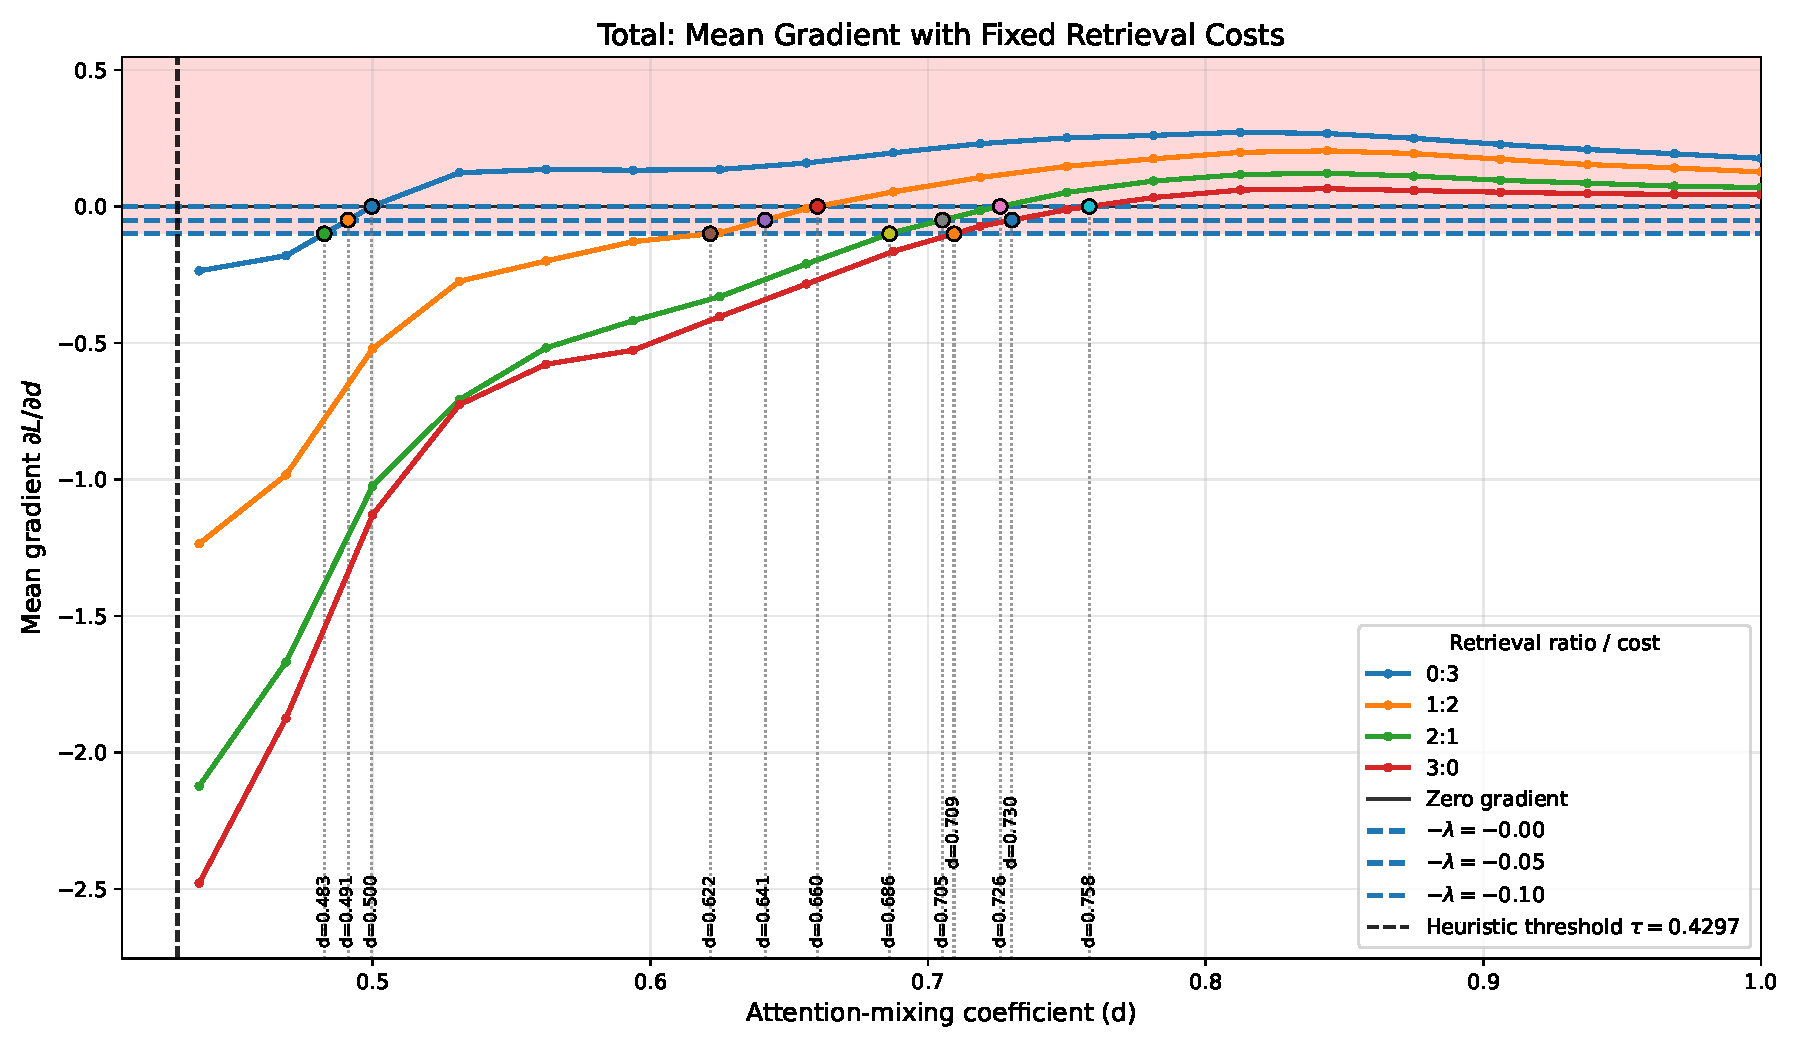
\includegraphics[width=\linewidth]{graphics/h2-cost.pdf}
\caption{H2: đối chiếu gradient với các mức \(-\lambda\). Nguồn: ô phân tích chi phí trong cùng notebook.}
\label{fig:h2cost}
\end{figure}
\clearpage
\subsection{Chất lượng hỏi đáp và tải truy hồi}
\begin{table}[htbp]\centering\small
\caption{Đối chứng địa phương, 500 mẫu mỗi bộ. ART dùng ngưỡng 0.4297. Chỉ số theo phần trăm.}
\label{tab:local}
\begin{tabular}{@{}llrrrl@{}}
\toprule
Bộ dữ liệu & Hệ thống & Acc & F1 & EM & ID \\
\midrule
MuSiQue & No-RAG & 0.80 & 5.61 & 0.60 & M05 \\
 & Vanilla RAG & 6.20 & 10.25 & 4.80 & M06 \\
 & ART & 25.80 & 31.17 & 21.60 & M12 \\
HotpotQA & No-RAG & 14.00 & 20.19 & 14.20 & M03 \\
 & Vanilla RAG & 33.20 & 39.61 & 30.20 & M04 \\
 & ART & 42.20 & 48.24 & 37.20 & M08 \\
2WikiMultiHopQA & No-RAG & 24.80 & 27.58 & 24.40 & M01 \\
 & Vanilla RAG & 34.80 & 37.81 & 32.20 & M02 \\
 & ART & 48.20 & 46.30 & 37.00 & M07 \\
\bottomrule
\end{tabular}
\end{table}

\Cref{tab:local} cho thấy ART ở ngưỡng mặc định cải thiện cả ba chỉ số trên cả ba bộ. So với Vanilla RAG, F1 tăng \(20.92\), \(8.63\), \(8.49\) điểm phần trăm theo thứ tự MuSiQue, HotpotQA, 2WikiMultiHopQA. So với No-RAG, mức tăng tương ứng là \(25.56\), \(28.05\), \(18.72\). Đây là kết quả của hệ thống hoàn chỉnh chứa cả quá trình tinh chỉnh và chính sách truy hồi.
\Cref{tab:sweep,fig:tradeoff} tóm tắt các cấu hình có ngưỡng xác định.
\begin{table}[htbp]\centering\small
\caption{Quét ngưỡng ART. TB là truy vấn/mẫu, Có (\%) là tỷ lệ mẫu có truy vấn và Tổng là số truy vấn ghi nhận.}
\label{tab:sweep}
\begin{tabular}{@{}lrrrrrrr@{}}
\toprule
Bộ dữ liệu & $\tau$ & Acc & F1 & EM & TB & Có (\%) & Tổng \\
\midrule
MuSiQue & 0.4297 & 25.80 & 31.17 & 21.60 & 4.792 & 100.0 & 2396 \\
 & 0.50 & 24.00 & 30.27 & 20.80 & 3.594 & 100.0 & 1797 \\
 & 0.60 & 26.00 & 32.08 & 22.80 & 2.588 & 100.0 & 1294 \\
 & 0.70 & 22.60 & 29.21 & 19.80 & 2.126 & 99.2 & 1063 \\
HotpotQA & 0.4297 & 42.20 & 48.24 & 37.20 & 4.070 & 100.0 & 2035 \\
 & 0.50 & 43.80 & 49.68 & 39.20 & 3.166 & 99.8 & 1583 \\
 & 0.60 & 40.00 & 46.87 & 36.40 & 2.278 & 99.2 & 1139 \\
2WikiMultiHopQA & 0.4297 & 48.20 & 46.30 & 37.00 & 4.012 & 100.0 & 2006 \\
 & 0.50 & 46.40 & 44.75 & 35.60 & 2.930 & 100.0 & 1465 \\
 & 0.60 & 44.40 & 44.34 & 36.00 & 2.126 & 99.4 & 1063 \\
\bottomrule
\end{tabular}
\end{table}


Retrieval count là số truy vấn ghi nhận trên mỗi mẫu hoàn tất, tính cả truy vấn lặp. Trên cả ba benchmark, số lượt trung bình giảm khi tăng \(\tau\) trong các cấu hình đã khảo sát. F1 giảm liên tiếp trên 2WikiMultiHopQA, tăng rồi giảm trên HotpotQA, và giảm, phục hồi rồi giảm lại trên MuSiQue. Chẳng hạn, MuSiQue ở ngưỡng \(0.60\) có 2.588 truy vấn trung bình và F1 32.08, so với 4.792 truy vấn và F1 31.17 ở cấu hình chuẩn. Ít truy vấn hơn có thể đi kèm F1 cao hơn hoặc thấp hơn tùy cấu hình. Số truy vấn phản ánh mức sử dụng truy hồi; các lượt chạy này không đo latency, FLOPs hay tổng compute.

\begin{figure}[htbp]\centering
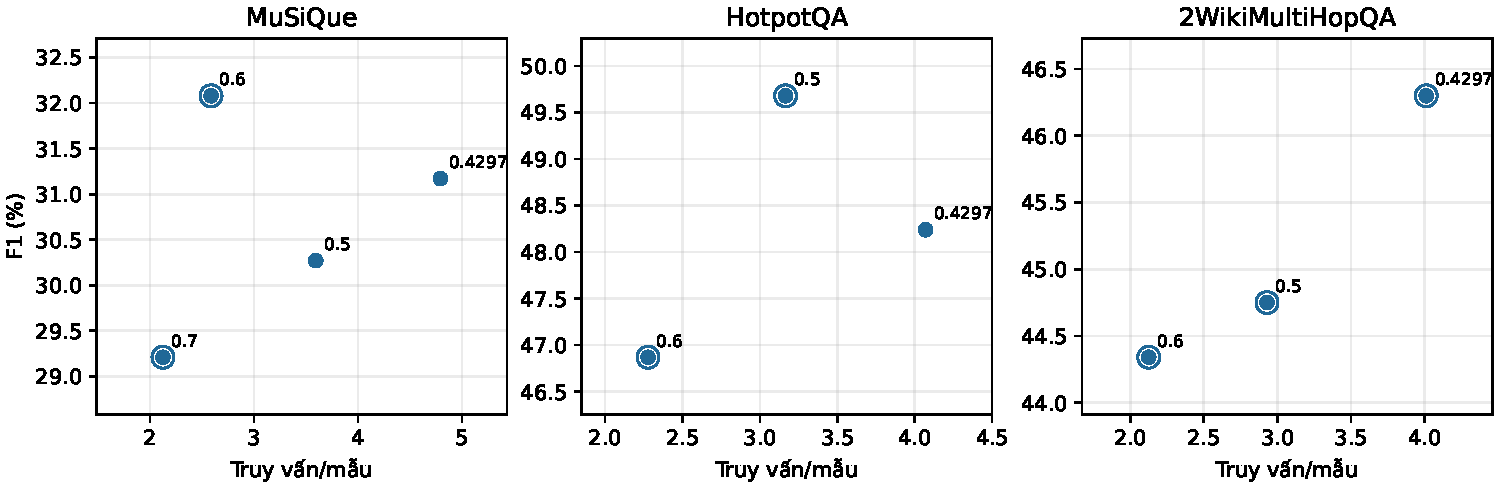
\includegraphics[width=\linewidth]{graphics/tradeoff.pdf}
\caption{F1 và số truy vấn trung bình trên các cấu hình có ngưỡng xác định. Các nhãn điểm là ngưỡng quyết định.}
\label{fig:tradeoff}
\end{figure}
\clearpage
\section{Thảo luận}
\subsection{Ví dụ đối sánh trên MuSiQue}
Ví dụ MuSiQue ID 348 ở \cref{fig:baseline-case} có EM bằng 0 với No-RAG và Vanilla RAG, và bằng 1 với ART. Đáp án của ART là \emph{Snapper Foster}. Phụ lục~\ref{app:examples} lưu nguyên văn các đầu ra và đoạn truy hồi.

Ở lượt đầu, đoạn \emph{Michael Knight (Knight Rider)} xác định David Hasselhoff là diễn viên. Lượt sau đưa tên David Hasselhoff vào truy vấn và trả về đoạn \emph{Snapper Foster}, nơi ghi rõ ông từng đóng vai này. Vanilla RAG có bằng chứng cho quan hệ đầu tiên trong năm đoạn đã lưu, nhưng thiếu đoạn xác nhận vai diễn. Chuỗi quan sát minh họa cách truy vấn được cập nhật theo thông tin đã tìm thấy. So sánh hệ thống này chưa cô lập ảnh hưởng của retrieval timing.

\subsection{So sánh cơ chế}
Các phương pháp IRCoT, Self-RAG và R-Search\cite{ircot,selfrag,rsearch} tiếp cận bài toán truy hồi thích nghi theo những cơ chế khác nhau. IRCoT kết hợp truy hồi với các bước suy luận trung gian; Self-RAG sử dụng các reflection tokens được học từ tín hiệu giám sát để điều khiển truy hồi; trong khi R-Search tối ưu quá trình tìm kiếm thông qua tín hiệu phần thưởng.

Khác với các phương pháp trên, ART kết hợp LM Loss với Retrieval Regularization trong cùng mục tiêu huấn luyện. Thông qua Attention Mixing, tín hiệu gradient từ quá trình dự đoán token có thể tác động gián tiếp đến Decision Head, giúp mô hình học cách điều chỉnh quyết định truy hồi mà không cần nhãn trực tiếp cho từng thời điểm truy hồi hoặc tối ưu chính sách bằng Reinforcement Learning. Tuy nhiên, ART vẫn sử dụng dữ liệu đích do teacher model tạo ra và quá trình Collect–Replay để tổ chức huấn luyện.

Kết quả thực nghiệm cho thấy hiệu quả của hệ thống ART hoàn chỉnh trên các bộ dữ liệu được khảo sát. Tuy nhiên, do ART sử dụng checkpoint đã fine-tune, trong khi các baseline sử dụng checkpoint gốc, kết quả hiện tại chưa tách biệt được đóng góp riêng của cơ chế lựa chọn thời điểm truy hồi. Để đánh giá riêng tác động này, cần thực hiện thêm các thí nghiệm ablation với checkpoint và điều kiện đánh giá tương thích.

\chapter{Kết luận và hướng phát triển}
\label{chap:conclusion}
\section{Kết luận}
Đồ án khảo sát cách học retrieval timing từ LM Loss và retrieval regularization. H1 cho thấy LM Loss nhạy với mức trộn và thành phần bằng chứng; H2 ghi nhận tín hiệu gradient hữu ích trong một số vùng. ART dùng Decision Head, Attention Mixing khả vi và Collect--Replay để học điểm mà không cần nhãn quyết định trực tiếp hay Reinforcement Learning.

Trên MuSiQue, HotpotQA và 2WikiMultiHopQA, ART tại \(\tau=0.4297\) cải thiện Acc, F1 và EM so với hai đối chứng địa phương. Trong threshold sweep, các ngưỡng cao hơn ghi nhận ít truy vấn hơn; thay đổi F1 phụ thuộc benchmark. Kết quả hệ thống và các probe bổ sung cho nhau khi đánh giá đóng góp của cơ chế học.

\section{Hạn chế}
Các probe cấp sẵn bằng chứng và dùng teacher forcing, nên chỉ xác nhận tín hiệu trong điều kiện khảo sát. So sánh hệ thống ghép cặp cùng câu hỏi nhưng chưa có ablation kiểm soát checkpoint và prompt để tách riêng hiệu ứng timing. Retrieval count đo hành vi gọi tìm kiếm; muốn đánh giá compute cần đo thêm độ dài ngữ cảnh, số token sinh và độ trễ thực tế.

\section{Hướng phát triển}
Có thể kiểm tra thêm bằng ngưỡng chọn trên tập xác thực và ablation giữ checkpoint cố định. Hai hướng Đồ án tốt nghiệp là khảo sát \emph{tool selection} theo trạng thái suy luận và huấn luyện chung retriever--generator để kiểm tra ảnh hưởng của tín hiệu sinh lên chất lượng bằng chứng.


\bibliographystyle{plain}
{\raggedright\bibliography{refs/references}}

\appendix
\chapter{Kết quả bổ sung}
\label{app:examples}
\section{Bản ghi đối sánh MuSiQue}
Ba dòng dữ liệu cùng mang ID 27, cùng câu hỏi và ground truth. ART dùng cấu hình top-5, \(\tau=0.4297\). Các raw outputs dưới đây giữ nguyên nội dung trước bước chấm điểm.

\begin{quote}\SingleSpacing
\textbf{Question}\par\nopagebreak[4]
{\small\ttfamily\raggedright
Who is the father of Nim\textquotesingle{}s actress in Return to Nim\textquotesingle{}s Island?\par
}
\textbf{Ground truth}\par\nopagebreak[4]
{\small\ttfamily\raggedright
Steve Irwin\par
}
\textbf{No-RAG}\par\nopagebreak[4]
{\small\ttfamily\raggedright
François Civil\textless{}\textbar{}im\_end\textbar{}\textgreater{}\par
}
\textbf{Vanilla RAG}\par\nopagebreak[4]
{\small\ttfamily\raggedright
John Wayne\textless{}\textbar{}im\_end\textbar{}\textgreater{}\par
}
\textbf{ART}\par\nopagebreak[4]
{\small\ttfamily\raggedright
To answer this question, we first need to identify the actress who played Nim in the film \textquotedbl{}Return to Nim\textquotesingle{}s Island.\textquotedbl{} AccordingThe document \textquotedbl{}Return to Nim\textquotesingle{}s Island\textquotedbl{} clearly states that Bindi Irwin played the role of Nim Rusoe. Therefore, Bindi Irwin is the actress we are looking for.\par
\par
Next, we need to determine the father of Bindi Irwin.The document \textquotedbl{}My Steve\textquotedbl{} provides information about Steve Irwin, stating that he was the father of Bindi Irwin. Therefore, the father of Nim\textquotesingle{}s actress in \textquotedbl{}Return to Nim\textquotesingle{}s Island\textquotedbl{} is Steve Irwin.\par
\par
\textless{}answer\textgreater{}\par
Steve Irwin\par
\textless{}/answer\textgreater{}\textless{}\textbar{}im\_end\textbar{}\textgreater{}\par
}

\end{quote}

\section{Truy vấn và tài liệu theo thứ tự ghi nhận}
No-RAG không có truy vấn hay tài liệu. Vanilla RAG ghi một truy vấn và năm đoạn; ART ghi hai truy vấn với năm đoạn mỗi lượt. Các mục dưới đây trích trực tiếp từ bản ghi. Chỉ lược bỏ những phần được đánh dấu.

\begin{quote}\SingleSpacing
\textbf{Vanilla RAG, query}\par\nopagebreak[4]
{\small\ttfamily\raggedright
Who did the actor who played Michael Knight play on Young and Restless?\par
}
\textbf{Vanilla RAG, passage 1}\par\nopagebreak[4]
{\small\ttfamily\raggedright
Title: Michael Baldwin\par
\textquotedbl{}Michael Baldwin\textquotedbl{}\par
Michael Baldwin is a fictional character from the CBS soap opera \textquotedbl{}The Young and the Restless\textquotedbl{}. The role is portrayed by Christian LeBlanc, originally from November 26, 1991 to July 7, 1993, and again since April 25, 1997.\par
}
\smallskip
\textbf{Vanilla RAG, passage 2}\par\nopagebreak[4]
{\small\ttfamily\raggedright
Title: Michael Knight (Knight Rider)\par
\textquotedbl{}Michael Knight (Knight Rider)\textquotedbl{}\par
Michael Knight is a fictional character and the protagonist of the 1980s television series \textquotedbl{}Knight Rider\textquotedbl{}, played by David Hasselhoff. The character first appeared in the opening scenes as Michael Long, played by Larry Anderson in the beginning of the pilot.\par
}
\smallskip
\textbf{Vanilla RAG, passage 3}\par\nopagebreak[4]
{\small\ttfamily\raggedright
Title: Robert Adamson (actor)\par
\textquotedbl{}Robert Adamson (actor)\textquotedbl{}\par
Robert Gillespie Adamson IV (born July 11, 1985) is an American actor. He has portrayed the roles of Phil Sanders on the television series Hollywood Heights and Charles Antoni on Lincoln Heights. He currently stars as Noah Newman on The Young and the Restless.\par
}
\smallskip
\textbf{Vanilla RAG, passage 4}\par\nopagebreak[4]
{\small\ttfamily\raggedright
Title: Michael Raymond-James\par
\textquotedbl{}Michael Raymond-James\textquotedbl{}\par
Michael Raymond - James (born Michael Weverstad; December 24, 1977) is an American actor. He is best known for playing René Lenier in the first season of the HBO series True Blood, Britt Pollack on the FX series Terriers, and Neal Cassidy / Baelfire on the ABC series Once Upon a Time.\par
}
\smallskip
\textbf{Vanilla RAG, passage 5}\par\nopagebreak[4]
{\small\ttfamily\raggedright
Title: Peter Bergman\par
\textquotedbl{}Peter Bergman\textquotedbl{}\par
Peter Michael Bergman (born June 11, 1953) is an American actor best known for his portrayals as Dr. Cliff Warner on All My Children (1979 -- 89) as well as Jack Abbott on The Young and the Restless (1989 -- present).\par
}
\smallskip
\textbf{ART, query 1}\par\nopagebreak[4]
{\small\ttfamily\raggedright
To answer this question, we first need to identify the actor who played Michael Knight.\par
}
\textbf{ART, query 1, passage 1}\par\nopagebreak[4]
{\small\ttfamily\raggedright
Title: Michael Knight (Knight Rider)\par
Michael Knight is a fictional character and the protagonist of the 1980s television series \textquotedbl{}Knight Rider\textquotedbl{}, played by David Hasselhoff. The character first appeared in the opening scenes as Michael Long, played by Larry Anderson in the beginning of the pilot.\par
}
\smallskip
\textbf{ART, query 1, passage 2}\par\nopagebreak[4]
{\small\ttfamily\raggedright
Title: Michael Raymond-James\par
Michael Raymond - James (born Michael Weverstad; December 24, 1977) is an American actor. He is best known for playing René Lenier in the first season of the HBO series True Blood, Britt Pollack on the FX series Terriers, and Neal Cassidy / Baelfire on the ABC series Once Upon a Time.\par
}
\smallskip
\textbf{ART, query 1, passage 3}\par\nopagebreak[4]
{\small\ttfamily\raggedright
Title: Michel Gill\par
Michel Gill (born April 16, 1960), also known as Michael Gill, is an American actor best known for playing President Garrett Walker in the Netflix series House of Cards and Gideon Goddard on Mr. Robot.\par
}
\smallskip
\textbf{ART, query 1, passage 4}\par\nopagebreak[4]
{\small\ttfamily\raggedright
Title: Christopher Knight (actor)\par
Christopher Anton Knight (born November 7, 1957) is an American actor, comedian and businessman. He is known for playing Peter Brady on the 1970s series \textquotedbl{}The Brady Bunch\textquotedbl{}. He has since gone on to become a successful businessman and enjoyed a semi-resurgence in the public eye with television appearances in the 2000s. His father, Edward Knight, was also an actor.\par
}
\smallskip
\textbf{ART, query 1, passage 5}\par\nopagebreak[4]
{\small\ttfamily\raggedright
Title: Michael Murphy (actor)\par
Michael George Murphy (born May 5, 1938) is an American film, television and stage actor. He often plays unethical or morally ambiguous characters in positions of authority, including politicians, executives and lawyers. He is also known for his frequent collaborations with director Robert Altman, having appeared in twelve films, TV series and miniseries directed by Altman from 1963 to 2004, including the title role in the miniseries \textquotedbl{}Tanner \textquotesingle{}88\textquotedbl{}.\par
}
\smallskip
\textbf{ART, query 2}\par\nopagebreak[4]
{\small\ttfamily\raggedright
Next, we need to determine who David Hasselhoff played on the television series \textquotedbl{}Young and Restless.\textquotedbl{}\par
}
\textbf{ART, query 2, passage 1}\par\nopagebreak[4]
{\small\ttfamily\raggedright
Title: Snapper Foster\par
Snapper Foster is a fictional character on the CBS daytime soap opera The Young and the Restless. An original character since the show\textquotesingle{}s inception, the role was played by William Gray Espy from March 26, 1973 to July 1975, and David Hasselhoff from 1975 to May 1982. Espy briefly reprised the character from February 28, 2003 to March 5, 2003, and Hasselhoff briefly reprised the role from June 15 -- 21, 2010.\par
}
\smallskip
\textbf{ART, query 2, passage 2}\par\nopagebreak[4]
{\small\ttfamily\raggedright
Title: Michael Knight (Knight Rider)\par
Michael Knight is a fictional character and the protagonist of the 1980s television series \textquotedbl{}Knight Rider\textquotedbl{}, played by David Hasselhoff. The character first appeared in the opening scenes as Michael Long, played by Larry Anderson in the beginning of the pilot.\par
}
\smallskip
\textbf{ART, query 2, passage 3}\par\nopagebreak[4]
{\small\ttfamily\raggedright
Title: Victor Newman\par
Victor Newman (born Christian Miller) is a fictional character from the American CBS soap opera The Young and the Restless. He has been portrayed by Eric Braeden since 1980. Initially a guest character who was to last for eight to twelve weeks, Victor has evolved into the soap opera\textquotesingle{}s leading male figure. Created by William J. Bell as a ``despicable, contemptible, unfaithful wife abuser \textquotesingle{}\textquotesingle{}, the character was planned to be killed off and never heard of again. However, after Bell saw Braeden\textquotesingle{}s performance, he decided to sign the actor onto a contract. Braeden was hesitant to work on a soap opera, but eventually signed a contract, and has remained on the series as a regular cast member for a total of thirty - seven years. The character is widely described as ruthless, and while loving to those he holds dear, is considered a villain. Over the years, he has also been the center of several controversial plots and relationships.\par
}
\smallskip
\textbf{ART, query 2, passage 4}\par\nopagebreak[4]
{\small\ttfamily\raggedright
Title: J. T. Hellstrom\par
J.T. Hellstrom is a fictional character from The Young and the Restless, an American soap opera on the CBS network. The role was portrayed by actor Thad Luckinbill from August 27, 1999, to November 5, 2010. Luckinbill originally appeared on a recurring basis until he was put on contract in November 2002. On November 3, 2017, it was announced that Luckinbill would reprise the role of J.T., beginning December 12, 2017.\par
}
\smallskip
\textbf{ART, query 2, passage 5}\par\nopagebreak[4]
{\small\ttfamily\raggedright
Title: Jerry Douglas (actor)\par
Jerry Douglas (born November 12, 1932) is an American television and film actor. For 25 years Jerry Douglas reigned in fictional Genoa City as patriarch John Abbott on the daytime television serial The Young and the Restless. In 2006, his character was killed off, however, he has made special appearances since then.\par
}
\smallskip

\end{quote}

Đoạn đầu lượt một nhận diện diễn viên, còn các đoạn 1 và 2 của lượt hai nối diễn viên với đáp án. Các đoạn trong cùng lượt được nhóm theo thứ tự top-5 trong log. Bản ghi cho biết tài liệu nào đã được truy hồi, chưa xác định được đoạn nào đã quyết định câu trả lời.

\chapter{Mã nguồn và khả năng tái lập}
\label{app:repro}
\section{Hiện vật và quy trình}
{\SingleSpacing\raggedright Mã nguồn của đồ án được công khai tại GitHub:\par
\url{https://github.com/nguyenphantuanduy/adaptive-retrieval-timing}.\par
Các tài nguyên phục vụ thực nghiệm và đánh giá, bao gồm checkpoint ART, dự kiến được công khai trên Hugging Face tại \url{https://huggingface.co/adaptive-retrieval-timing}.\par}

Kết quả dự đoán và các chỉ số đánh giá của ART được lưu tại \path{art-backup/demo-3}, trong khi kết quả của các phương pháp đối chứng được lưu tại \path{REVIVE_training/result/baselines}. Các bảng, hình minh họa và ví dụ phân tích được tái tạo từ những tệp kết quả đã lưu, theo quy trình mô tả trong \path{docs/report_execution/REVIEW_2026-11-22.md}.

Một số checkpoint và chỉ mục truy hồi từ các lần thực nghiệm trước chưa được ghi nhận bằng revision bất biến. Do đó, khả năng tái lập chính xác các lần chạy lịch sử vẫn phụ thuộc vào tính sẵn có của những hiện vật tương ứng.

\section{Giới hạn của phép đếm tải huấn luyện}
{\SingleSpacing
Với khoảng 20\,000 mẫu và \(0.75\) epoch, phép nhân cho khoảng 15\,000 lượt trình bày đích giáo viên cho student. Phép đếm này dựa trên kích thước tập xấp xỉ; nó chưa bao gồm một lượt sinh đích bằng Qwen3-8B, số token, truy hồi trong Collect và việc chạy lại các tiền tố trong Replay.

Để minh họa một đơn vị đếm khác, cấu hình R-Search công bố tối đa 195 bước, batch 256 và năm phản hồi mỗi prompt\cite{rsearch}. Nếu đủ 195 bước và 256 prompt mỗi bước, phép nhân \(195\times256\times5=249\,600\) cho số phản hồi theo kịch bản. Tỷ số số đếm khoảng \(6\%\) chỉ tái hiện phép tính dưới giả định đó. Lượt trình bày đích và lượt rollout là hai đơn vị khác nhau; rollout còn có generation, tìm kiếm và chấm reward. Thiếu số đo chung về GPU-hours, FLOPs và latency để ước lượng chênh lệch tổng compute.\par}


\end{document}
